
\section{Extreme Learning Machines}
Extreme Learning Machines, 2006 yılında Guang-Bin Huang ve arkadaşları tarafından önerilmiştir. Tek gizli katmana sahiptir. Geleneksel sinir ağlarından farklı olarak, gizli katmandaki nöronların ağırlıklarının rastgele atanması ve sadece çıktı katmanındaki ağırlıkların eğitilmesidir.

\begin{figure}[h]
    \centering
    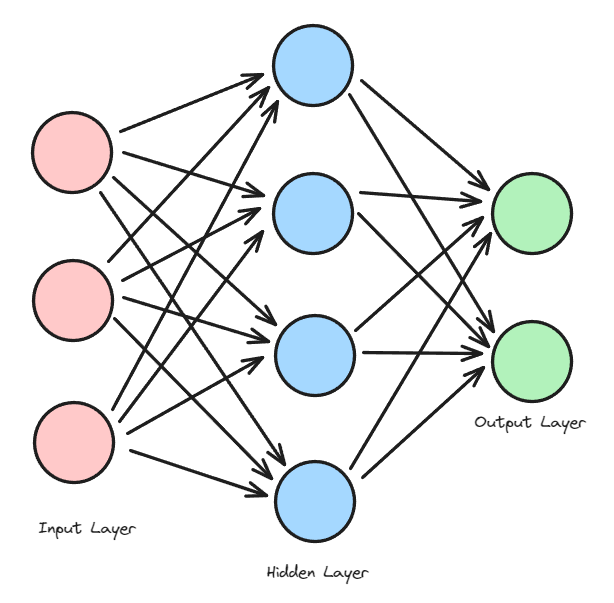
\includegraphics[width=0.7\textwidth]{images/extreme_learning_machine.png}
    \caption{Aşırı öğrenme makinesi mimarisi.}
    \label{fig:enter-label}
\end{figure}

\subsection{Çalışma Adımları}
\begin{enumerate}
    \item Giriş özellikleri ve gizli katmandaki nöronlar arasındaki bağlantı ağırlıkları rastgele atanır.
    \item Giriş özelliklerini gizli katmandaki nöronlara iletmek için bir aktivasyon oluşturulur.
    \item Aktivasyonlar, gizli katmandaki nöronlarla çıkış katmanındaki nöronlar arasındaki ağırlıklar ile çarpılır. Bu çarpımların ortalaması alınarak çıkış katmanındaki nöronların ağırlıkları belirlenir.
    \item Çıkış katmanındaki nöronlar, aktivasyonların ağırlıklarla çarpımının toplamını alır ve aktivasyon fonksiyonundan geçirerek çıkış üretir.
\end{enumerate}

\newpage